\begin{table}[ht]
\centering\small
\caption{Common-query performance. Mean and 95\% seed-cluster bootstrap interval for excess cost, mean retained \emph{scalar data inequalities} (prior excluded), and mean total milliseconds per query including archive refinement. Fixed-budget methods retain whole transitions.}\label{tab:main}
\begin{tabular}{llrrrr}\toprule
Plant $(n,m)$ & Method & Mean gap & 95\% interval & Data & ms\\\midrule
Thermal (4,2) & DCC ($10^{-5}$) & 2.53e-08 & [9.8e-09,4.4e-08] & 31.8 & 25.9 \\
 & DCC ($10^{-3}$) & 1.05e-05 & [8.6e-06,1.2e-05] & 31.7 & 22.5 \\
 & Random & 1.42e-02 & [1.2e-02,1.7e-02] & 384.0 & 6.1 \\
 & Log-det & 8.97e-03 & [7.7e-03,1.0e-02] & 384.0 & 6.1 \\
 & Window & 1.57e-02 & [1.2e-02,1.9e-02] & 384.0 & 6.0 \\
 & Prior & 2.43e-01 & [2.3e-01,2.6e-01] & 0.0 & 4.1 \\
\midrule
Mechanical (4,2) & DCC ($10^{-5}$) & 4.57e-09 & [-4.3e-18,1.2e-08] & 14.8 & 13.2 \\
 & DCC ($10^{-3}$) & 4.16e-06 & [1.1e-06,8.1e-06] & 13.4 & 12.4 \\
 & Random & 9.80e-03 & [8.6e-03,1.1e-02] & 384.0 & 4.4 \\
 & Log-det & 7.84e-03 & [6.1e-03,9.7e-03] & 384.0 & 4.5 \\
 & Window & 1.10e-02 & [9.2e-03,1.3e-02] & 384.0 & 4.3 \\
 & Prior & 4.98e-02 & [4.6e-02,5.5e-02] & 0.0 & 3.4 \\
\midrule
Nonnormal (6,2) & DCC ($10^{-5}$) & 5.23e-09 & [1.0e-09,9.9e-09] & 59.5 & 63.1 \\
 & DCC ($10^{-3}$) & 1.31e-05 & [1.0e-05,1.6e-05] & 59.3 & 55.6 \\
 & Random & 2.43e-02 & [2.3e-02,2.6e-02] & 1152.0 & 17.3 \\
 & Log-det & 1.89e-02 & [1.7e-02,2.0e-02] & 1152.0 & 17.2 \\
 & Window & 2.61e-02 & [2.5e-02,2.8e-02] & 1152.0 & 17.0 \\
 & Prior & 1.71e-01 & [1.6e-01,1.8e-01] & 0.0 & 9.1 \\
\midrule
Dense (8,3) & DCC ($10^{-5}$) & 8.97e-10 & [-1.9e-17,2.7e-09] & 71.7 & 15.4 \\
 & DCC ($10^{-3}$) & 3.81e-08 & [3.3e-18,1.1e-07] & 71.7 & 15.1 \\
 & Random & 2.62e-03 & [2.0e-03,3.4e-03] & 2816.0 & 20.0 \\
 & Log-det & 2.19e-03 & [1.5e-03,3.1e-03] & 2816.0 & 19.9 \\
 & Window & 2.31e-03 & [1.8e-03,3.0e-03] & 2816.0 & 19.5 \\
 & Prior & 2.39e-02 & [1.9e-02,2.8e-02] & 0.0 & 4.9 \\
\bottomrule\end{tabular}
\end{table}
\begin{figure}[ht]
\centering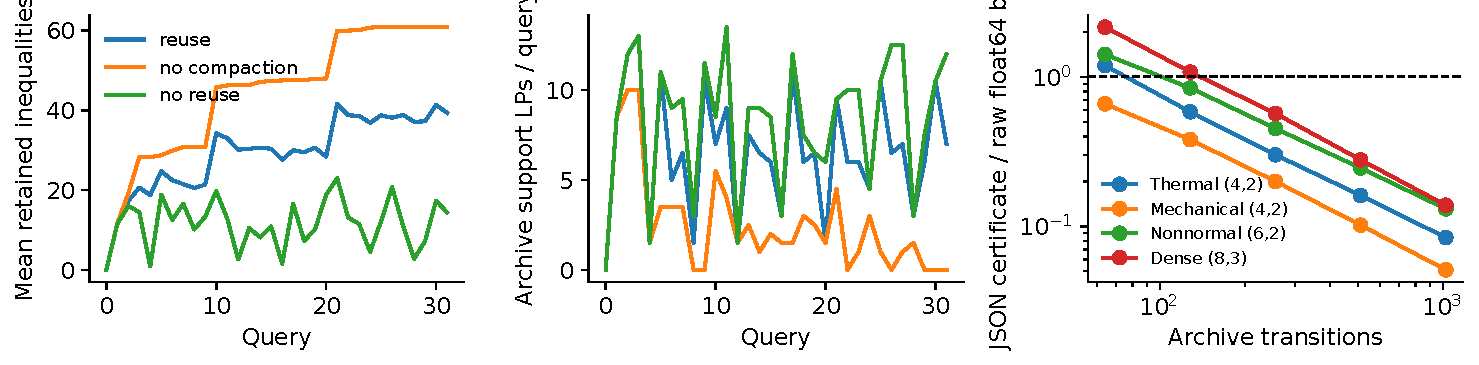
\includegraphics[width=\linewidth]{figures/ablation_streaming.pdf}
\caption{Ablations and streaming. Compaction limits retained data; reuse can reduce archive support calls relative to restarting. Payload ratios compare complete serialized controller certificates, including prior constraints and row witnesses, with raw transition arrays in float64. They are representation-size proxies, not measured network traffic or process memory.}\label{fig:ablation}
\end{figure}
\subsection{Stale-witness counterexample}
A scalar example isolates this issue without restricting the main method. Let $A=0$, $B\in[0.5,1.5]$, $\eta=0.1$, $x=0$, $v=1$, and $\bar u=0.8$. The old transition $(u,y)=(0.1,0.1)$ does not tighten the prior. The safe action is $0.6$, with cost $0.08$; the feasible old witness $B=1.5$ gives the same optimistic cost. A new transition $(u,y)=(1,0.5)$ restricts $B$ to $[0.5,0.6]$. The new full-data action is $0.8$, with cost $0.02$. Unscreened reuse would certify zero gap for a decision whose actual gap is $0.06$. The new transition can be collected in a separate identification experiment; it is not claimed to satisfy the later deployment input bound. The supplied executable example reproduces the numbers including numerical margins.

\subsection{Proof of Proposition~\ref{prop:polygon}}
\begin{proof}
For any $N\geq4$, let $z_j=(\cos(j\pi/N),\sin(j\pi/N))$, $j=0,\ldots,N-1$, $y_j=0$, $\eta=1$, and prior $[-3,3]^2$. The true row parameter is zero. Independently reset one-step experiments realize these regressors and zero disturbances. Each slab $|z_j^\top\theta|\leq1$ defines two distinct sides of a regular $2N$-gon. Removing that transition increases the support in direction $z_j$, since the adjacent facet intersections lie strictly beyond its removed side. All $N$ transitions are thus necessary for exact uniform support preservation.
\end{proof}
